% Options for packages loaded elsewhere
\PassOptionsToPackage{unicode}{hyperref}
\PassOptionsToPackage{hyphens}{url}
%
\documentclass[
  ignorenonframetext,
]{beamer}
\usepackage{pgfpages}
\setbeamertemplate{caption}[numbered]
\setbeamertemplate{caption label separator}{: }
\setbeamercolor{caption name}{fg=normal text.fg}
\beamertemplatenavigationsymbolsempty
% Prevent slide breaks in the middle of a paragraph
\widowpenalties 1 10000
\raggedbottom
\setbeamertemplate{part page}{
  \centering
  \begin{beamercolorbox}[sep=16pt,center]{part title}
    \usebeamerfont{part title}\insertpart\par
  \end{beamercolorbox}
}
\setbeamertemplate{section page}{
  \centering
  \begin{beamercolorbox}[sep=12pt,center]{part title}
    \usebeamerfont{section title}\insertsection\par
  \end{beamercolorbox}
}
\setbeamertemplate{subsection page}{
  \centering
  \begin{beamercolorbox}[sep=8pt,center]{part title}
    \usebeamerfont{subsection title}\insertsubsection\par
  \end{beamercolorbox}
}
\AtBeginPart{
  \frame{\partpage}
}
\AtBeginSection{
  \ifbibliography
  \else
    \frame{\sectionpage}
  \fi
}
\AtBeginSubsection{
  \frame{\subsectionpage}
}

\usepackage{amsmath,amssymb}
\usepackage{lmodern}
\usepackage{iftex}
\ifPDFTeX
  \usepackage[T1]{fontenc}
  \usepackage[utf8]{inputenc}
  \usepackage{textcomp} % provide euro and other symbols
\else % if luatex or xetex
  \usepackage{unicode-math}
  \defaultfontfeatures{Scale=MatchLowercase}
  \defaultfontfeatures[\rmfamily]{Ligatures=TeX,Scale=1}
\fi
% Use upquote if available, for straight quotes in verbatim environments
\IfFileExists{upquote.sty}{\usepackage{upquote}}{}
\IfFileExists{microtype.sty}{% use microtype if available
  \usepackage[]{microtype}
  \UseMicrotypeSet[protrusion]{basicmath} % disable protrusion for tt fonts
}{}
\makeatletter
\@ifundefined{KOMAClassName}{% if non-KOMA class
  \IfFileExists{parskip.sty}{%
    \usepackage{parskip}
  }{% else
    \setlength{\parindent}{0pt}
    \setlength{\parskip}{6pt plus 2pt minus 1pt}}
}{% if KOMA class
  \KOMAoptions{parskip=half}}
\makeatother
\usepackage{xcolor}
\geometry{tmargin=0em}
\newif\ifbibliography
\setlength{\emergencystretch}{3em} % prevent overfull lines
\setcounter{secnumdepth}{-\maxdimen} % remove section numbering


\providecommand{\tightlist}{%
  \setlength{\itemsep}{0pt}\setlength{\parskip}{0pt}}\usepackage{longtable,booktabs,array}
\usepackage{calc} % for calculating minipage widths
\usepackage{caption}
% Make caption package work with longtable
\makeatletter
\def\fnum@table{\tablename~\thetable}
\makeatother
\usepackage{graphicx}
\makeatletter
\def\maxwidth{\ifdim\Gin@nat@width>\linewidth\linewidth\else\Gin@nat@width\fi}
\def\maxheight{\ifdim\Gin@nat@height>\textheight\textheight\else\Gin@nat@height\fi}
\makeatother
% Scale images if necessary, so that they will not overflow the page
% margins by default, and it is still possible to overwrite the defaults
% using explicit options in \includegraphics[width, height, ...]{}
\setkeys{Gin}{width=\maxwidth,height=\maxheight,keepaspectratio}
% Set default figure placement to htbp
\makeatletter
\def\fps@figure{htbp}
\makeatother

\usepackage{booktabs}
\usepackage{longtable}
\usepackage{array}
\usepackage{multirow}
\usepackage{wrapfig}
\usepackage{float}
\usepackage{colortbl}
\usepackage{pdflscape}
\usepackage{tabu}
\usepackage{threeparttable}
\usepackage{threeparttablex}
\usepackage[normalem]{ulem}
\usepackage{makecell}
\usepackage{xcolor}
\makeatletter
\makeatother
\makeatletter
\makeatother
\makeatletter
\@ifpackageloaded{caption}{}{\usepackage{caption}}
\AtBeginDocument{%
\ifdefined\contentsname
  \renewcommand*\contentsname{Table of contents}
\else
  \newcommand\contentsname{Table of contents}
\fi
\ifdefined\listfigurename
  \renewcommand*\listfigurename{List of Figures}
\else
  \newcommand\listfigurename{List of Figures}
\fi
\ifdefined\listtablename
  \renewcommand*\listtablename{List of Tables}
\else
  \newcommand\listtablename{List of Tables}
\fi
\ifdefined\figurename
  \renewcommand*\figurename{Figure}
\else
  \newcommand\figurename{Figure}
\fi
\ifdefined\tablename
  \renewcommand*\tablename{Table}
\else
  \newcommand\tablename{Table}
\fi
}
\@ifpackageloaded{float}{}{\usepackage{float}}
\floatstyle{ruled}
\@ifundefined{c@chapter}{\newfloat{codelisting}{h}{lop}}{\newfloat{codelisting}{h}{lop}[chapter]}
\floatname{codelisting}{Listing}
\newcommand*\listoflistings{\listof{codelisting}{List of Listings}}
\makeatother
\makeatletter
\@ifpackageloaded{caption}{}{\usepackage{caption}}
\@ifpackageloaded{subcaption}{}{\usepackage{subcaption}}
\makeatother
\makeatletter
\@ifpackageloaded{tcolorbox}{}{\usepackage[many]{tcolorbox}}
\makeatother
\makeatletter
\@ifundefined{shadecolor}{\definecolor{shadecolor}{rgb}{.97, .97, .97}}
\makeatother
\makeatletter
\makeatother
\ifLuaTeX
  \usepackage{selnolig}  % disable illegal ligatures
\fi
\IfFileExists{bookmark.sty}{\usepackage{bookmark}}{\usepackage{hyperref}}
\IfFileExists{xurl.sty}{\usepackage{xurl}}{} % add URL line breaks if available
\urlstyle{same} % disable monospaced font for URLs
\hypersetup{
  pdftitle={How Heterogeneity Impacts Learning},
  hidelinks,
  pdfcreator={LaTeX via pandoc}}

\title{How Heterogeneity Impacts Learning}
\author{Hossein Alidaee}
\date{}

\begin{document}

\frame{\titlepage}
\ifdefined\Shaded\renewenvironment{Shaded}{\begin{tcolorbox}[enhanced, interior hidden, borderline west={3pt}{0pt}{shadecolor}, sharp corners, frame hidden, breakable, boxrule=0pt]}{\end{tcolorbox}}\fi

\begin{frame}{Motivation}
\protect\hypertarget{motivation}{}
\end{frame}

\begin{frame}{Social Learning Is Oddly Influential}
\protect\hypertarget{social-learning-is-oddly-influential}{}
Peers have limited experience

Authorities test recommendations extensively

Yet, both induce adoption at equal rates

\begin{itemize}
\tightlist
\item
  Krishnan and Patnam (2013)
\item
  Takahashi, Mano, and Otsuka (2019)
\end{itemize}

Implies social learning is more influential \emph{per data point}
\end{frame}

\begin{frame}{What's the mechanism?}
\protect\hypertarget{whats-the-mechanism}{}
Natural questions:

\begin{itemize}[<+->]
\tightlist
\item
  \textbf{Why?}
\item
  \textbf{Is social learning special?}
\item
  \textbf{How can authorities improve?}
\end{itemize}
\end{frame}

\begin{frame}{My Proposal: Context Uncertainty}
\protect\hypertarget{my-proposal-context-uncertainty}{}
Peer information comes with rich context

Information from authorities comes with little context

When weighing signals, we place weight on total uncertainty

Total Uncertainty = Context Uncertainty + Sampling Error
\end{frame}

\begin{frame}{Related Literature}
\protect\hypertarget{related-literature}{}
\begin{itemize}
\tightlist
\item
  Decision makers as statisticians

  \begin{itemize}
  \tightlist
  \item
    Steiner and Stewart (2008), Olea et al.~(2021), Salant and Cherry
    (2020), etc..
  \end{itemize}
\item
  Social learning theory

  \begin{itemize}
  \tightlist
  \item
    Sethi and Yildiz (2016), Dasaratha et al (2022), Bala and Goyal
    (1998), etc\ldots{}
  \end{itemize}
\item
  Information provision experiments

  \begin{itemize}
  \tightlist
  \item
    Jensen (2010), Chetty and Saez (2013), Binder (2020), etc\ldots{}
  \end{itemize}
\item
  Role of heterogeneity in agents' responses to information

  \begin{itemize}
  \tightlist
  \item
    Armour (2018),
  \end{itemize}
\item
  Role of trust in agents' responses to information

  \begin{itemize}
  \tightlist
  \item
    asdf
  \end{itemize}
\item
  Agricultural technology adoption

  \begin{itemize}
  \tightlist
  \item
    asdf
  \end{itemize}
\item
  Agricultural extension design

  \begin{itemize}
  \tightlist
  \item
    asdf
  \end{itemize}
\end{itemize}
\end{frame}

\begin{frame}{Roadmap}
\protect\hypertarget{roadmap}{}
Today:

\begin{itemize}[<+->]
\tightlist
\item
  Relate question to agricultural technology adoption
\item
  Propose a foundation for mechanism
\item
  Provide experimental design
\item
  Present results
\item
  Discuss external validity
\item
  Implications for farmers and policymakers
\item
  Upcoming extensions
\end{itemize}
\end{frame}

\begin{frame}{Setting}
\protect\hypertarget{setting}{}
\end{frame}

\begin{frame}{Low AgTech Adoption Is A Major Issue}
\protect\hypertarget{low-agtech-adoption-is-a-major-issue}{}
\begin{columns}[T]
\begin{column}{0.55\textwidth}
\begin{figure}

\hfill{} 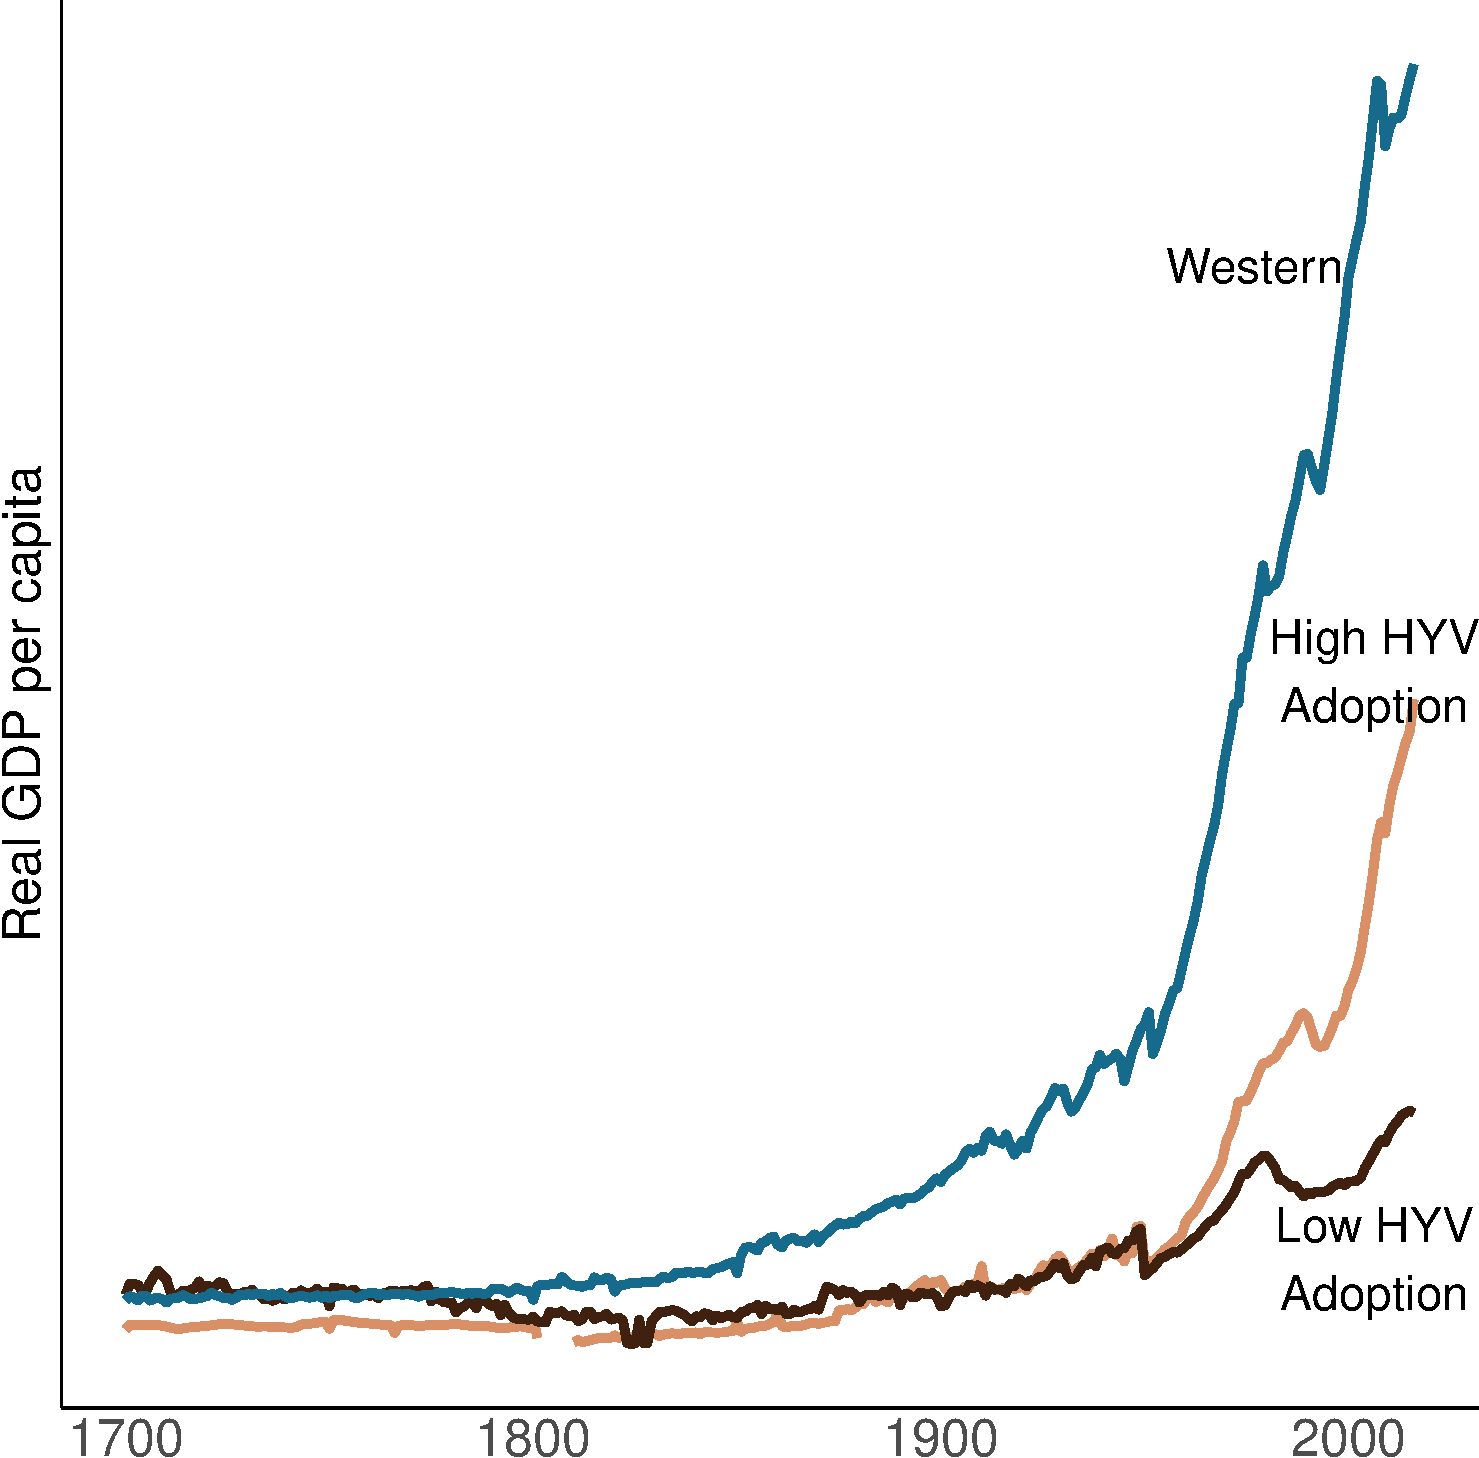
\includegraphics{presentation_lori_files/figure-beamer/unnamed-chunk-2-1.pdf}

\end{figure}
\end{column}

\begin{column}{0.35\textwidth}
\begin{itemize}[<+->]
\tightlist
\item
  \(2^{\text{nd}}\) divergence via Green Revolution (Huang, 2020)
\end{itemize}

\begin{itemize}[<+->]
\tightlist
\item
  Key friction for AgTech (Magruder, 2018)
\end{itemize}

\begin{itemize}[<+->]
\tightlist
\item
  Governments spend huge sums on extension (Akroyd and Smith, 2007)
\end{itemize}
\end{column}
\end{columns}
\end{frame}

\begin{frame}{Traditional Extension Design}
\protect\hypertarget{traditional-extension-design}{}
\begin{itemize}[<+->]
\tightlist
\item
  R\&D at university or national research institute
\item
  Pick a winning technology
\item
  Agricultural ministry teaches extension staff
\item
  Extension staff advocate in villages
\item
  Villagers have no clue about test conditions
\end{itemize}

\begin{figure}

\begin{minipage}[t]{0.20\linewidth}

{\centering 

\raisebox{-\height}{

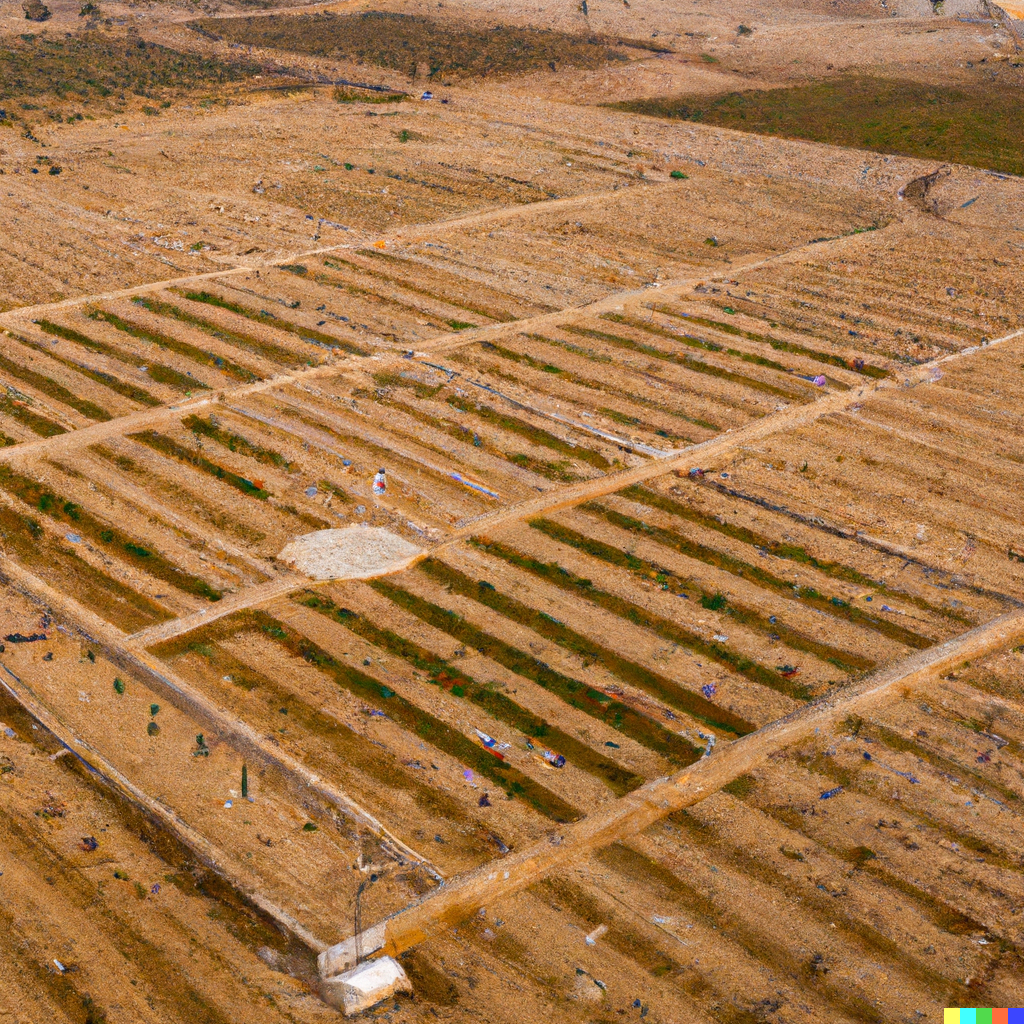
\includegraphics[width=3.125in,height=\textheight]{generic_extension.png}

}

}

\end{minipage}%
%
\begin{minipage}[t]{0.20\linewidth}

{\centering 

\raisebox{-\height}{

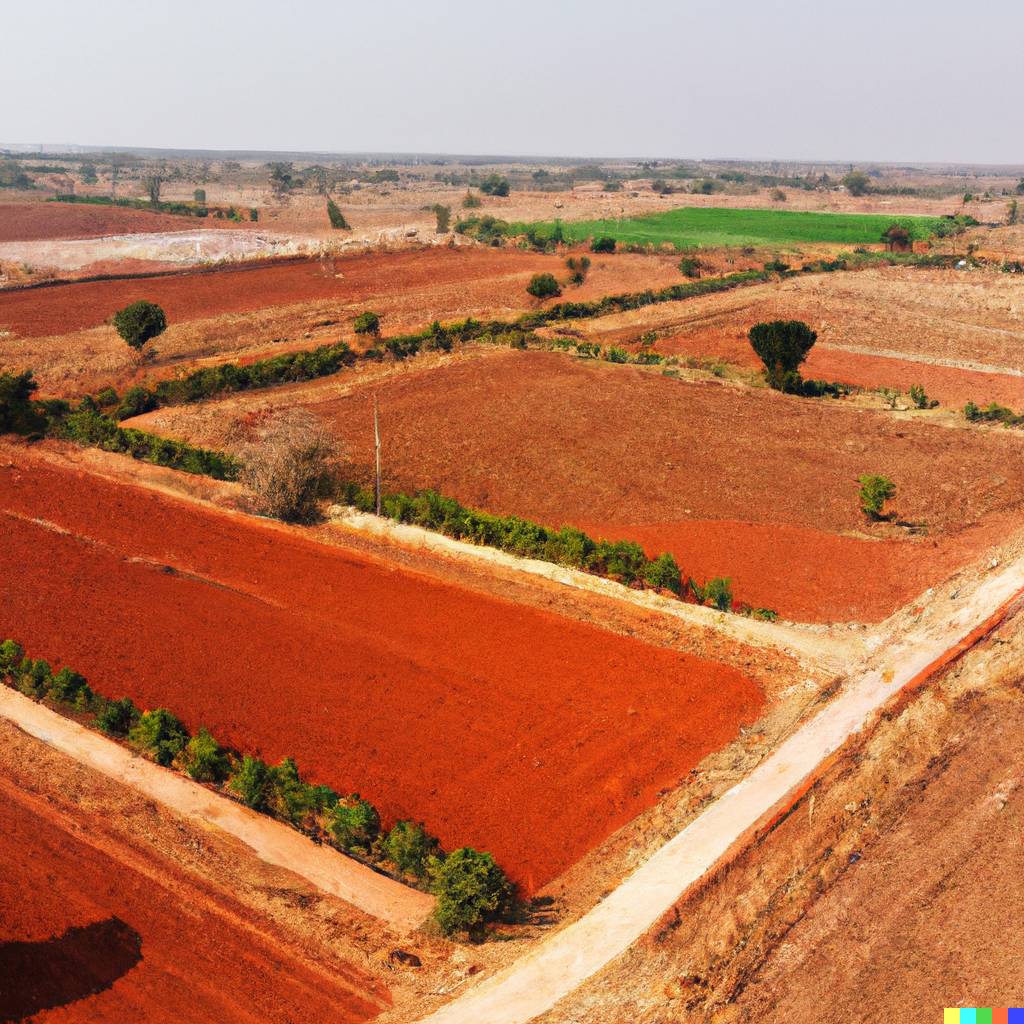
\includegraphics[width=3.125in,height=\textheight]{redsoil_extension.png}

}

}

\end{minipage}%
%
\begin{minipage}[t]{0.20\linewidth}

{\centering 

\raisebox{-\height}{

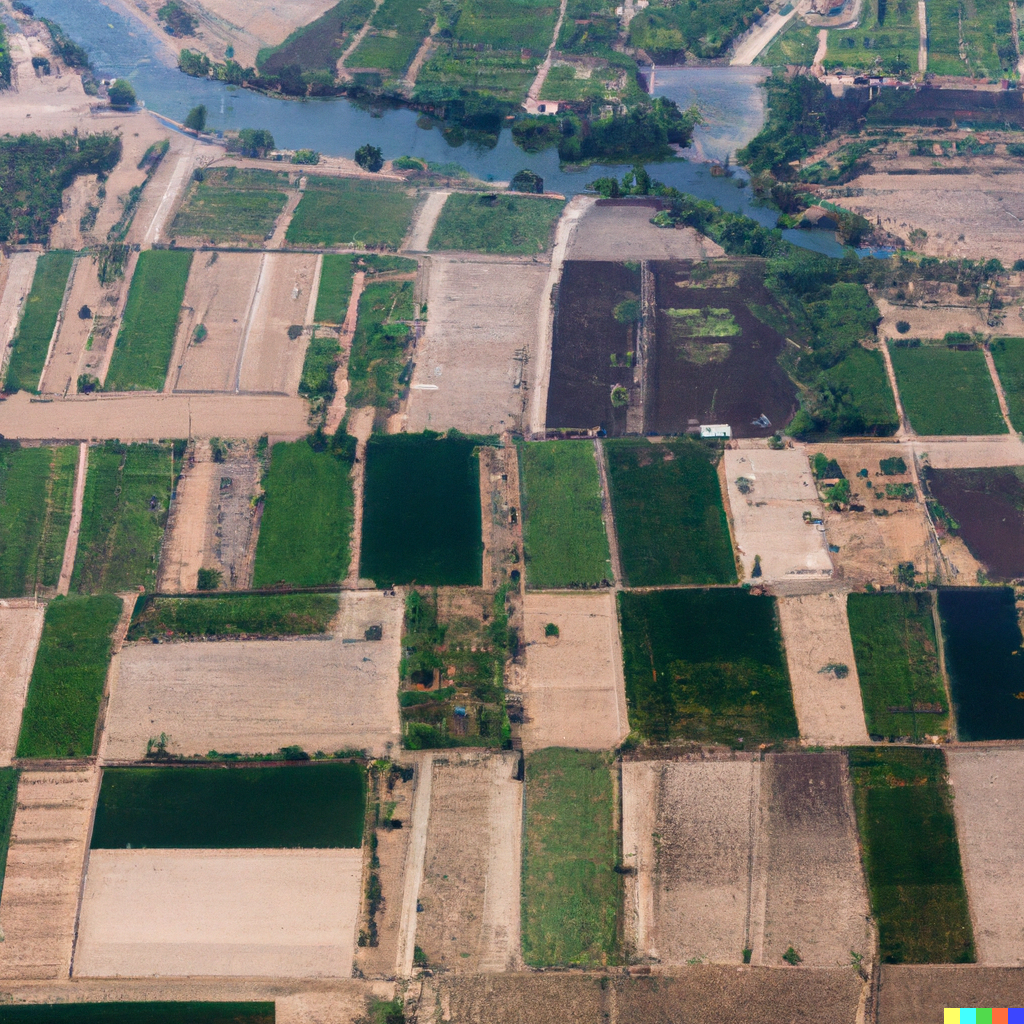
\includegraphics[width=3.125in,height=\textheight]{riverbed_extension.png}

}

}

\end{minipage}%
%
\begin{minipage}[t]{0.20\linewidth}

{\centering 

\raisebox{-\height}{

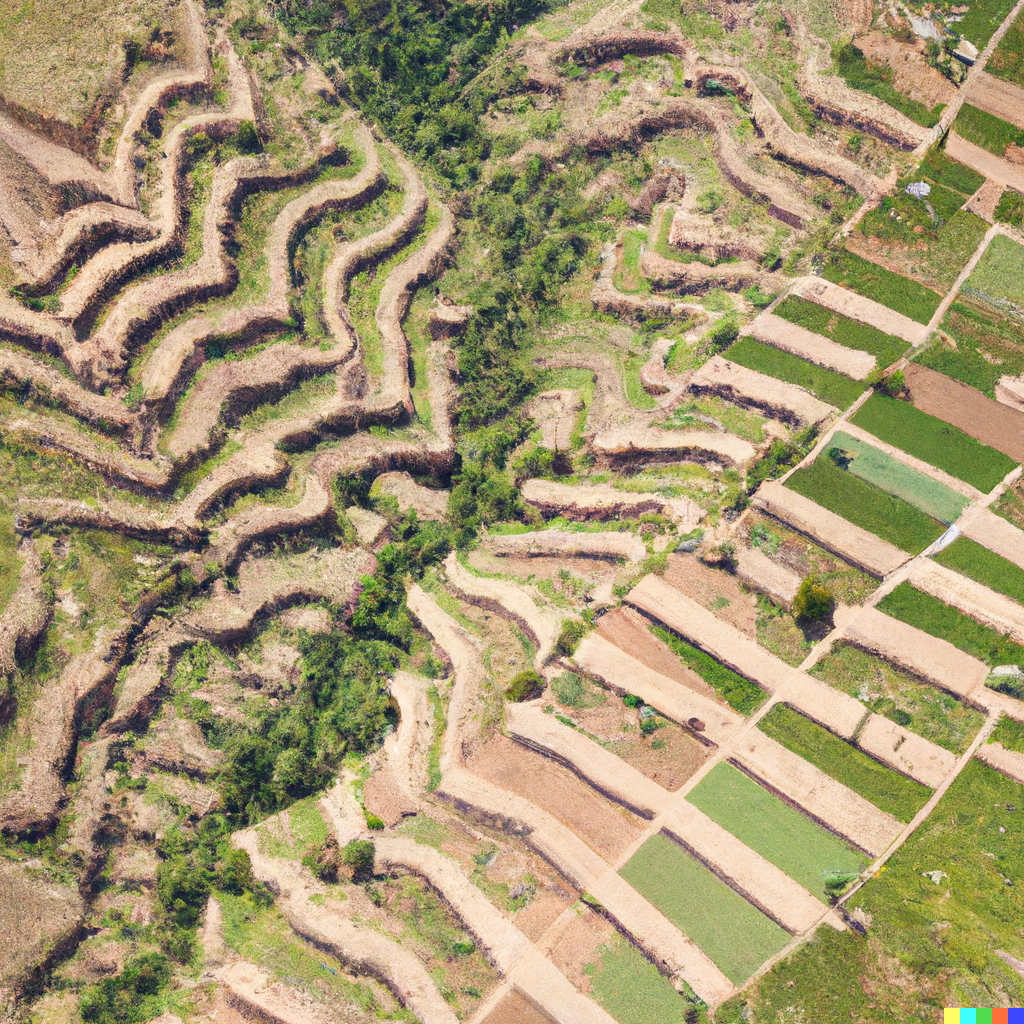
\includegraphics[width=3.125in,height=\textheight]{hillside_extension.png}

}

}

\end{minipage}%
%
\begin{minipage}[t]{0.20\linewidth}

{\centering 

\raisebox{-\height}{

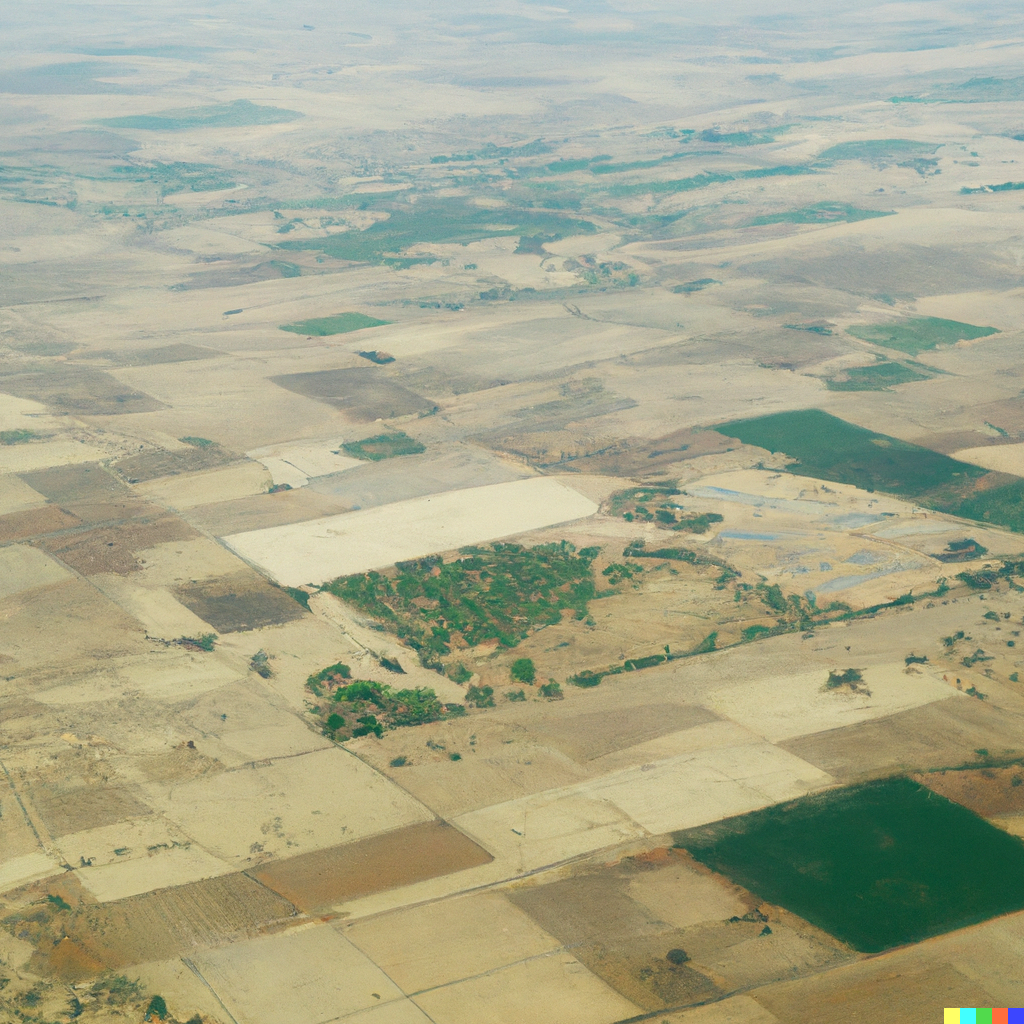
\includegraphics[width=3.125in,height=\textheight]{drylands_extension.png}

}

}

\end{minipage}%

\end{figure}
\end{frame}

\begin{frame}{Microfoundation}
\protect\hypertarget{microfoundation}{}
\end{frame}

\begin{frame}{The Farmer's Problem}
\protect\hypertarget{the-farmers-problem}{}
\textbf{Problem:}

\[ 
\operatorname*{argmax}_\alpha E[U(\alpha \cdot \theta_i ) | s_1, \ldots s_n, s_E]
\]

\textbf{Decision:} Fraction of investment \(\alpha \in [0, 1]\)

\textbf{Heterogeneity:}

\[
\ \ \ \ \ \ \ \ \ \ \ \ \theta_i = \underbrace{\theta \vphantom{\gamma_i}  }_{\text{average return}} + \underbrace{\gamma_i}_{\text{context adjustment}}
\]

\textbf{Belief:} Posterior \(\tilde{\theta}_i\)

\textbf{Preferences:} Risk averse so

\[
\ \ \ \ \ \ \ \ \ \ \ \ \ \ \ \ \ \ \ \ \ \ \ \ \ \ \ \ \ \ \ \ \ \ \ \  \operatorname{E}[U(\alpha \theta_i)] \leq U(\alpha  \operatorname{E}[\theta_i]).
\]
\end{frame}

\begin{frame}{Interpreting Signals from peers}
\protect\hypertarget{interpreting-signals-from-peers}{}
Friend \(j\) shares signal \[
s_j = \underbrace{\theta\vphantom{\gamma_j}}_{\text{Average Return}} + \underbrace{\gamma_j}_{\text{Agent $j$'s Context}} + \underbrace{\epsilon_j}_{\text{Agent $j$'s Sampling Error}}.
\]

Farmer's belief about \(\gamma_j\) is \[
\gamma_j \sim \mathcal{N}\left(0, (\sigma_j^\gamma)^2\right).
\]

Farmer knows friend \(j\) well, so context uncertainty
\(\sigma_j^\gamma\) is low.
\end{frame}

\begin{frame}{Interpreting Signals from Authorities}
\protect\hypertarget{interpreting-signals-from-authorities}{}
Extension agent \(E\) shares signal \[
s_E = \underbrace{\theta\vphantom{\gamma_E}}_{\text{Average Return}} + \underbrace{\gamma_E}_{\text{Agent's Context}} + \underbrace{\epsilon_E}_{\text{Agent's Sampling Error}}.
\]

Farmer's belief about \(\gamma_E\) is \[
\gamma_E \sim \mathcal{N}\left(0, (\sigma_E^\gamma)^2\right).
\]

Farmer doesn't know any context, so \(\sigma_E^\gamma\) is high.
\end{frame}

\begin{frame}{Adjusting Signals for Context}
\protect\hypertarget{adjusting-signals-for-context}{}
How does the farmer adapt the signal to his own context?

\[\begin{aligned}
\text{Adjusted Signal} &= \text{Original Signal} \\
& \ \ \  + \text{Own Context Adjustment} \\
& \ \ \  - \text{Friend's Context Adjustment}
\end{aligned}\]

\textbf{Implication:}

↑ context uncertainty ⇒ ↑ variance in adjusted signal
\end{frame}

\begin{frame}{Our Farmer's Posterior}
\protect\hypertarget{our-farmers-posterior}{}
Using information from all sources, farmer updates his belief.

\[\begin{aligned}
\text{Mean} &\propto \frac{0}{\text{Prior Var}}  + \frac{\text{Ext Adj Signal}}{\text{Ext Sample Var} + \text{Ext Context Var}} \\
 & \ \ \ \ + \sum \frac{\text{Peer Adj Signal}}{\text{Peer Sample Var} + \text{Peer Context Var}} 
\end{aligned}\]
\end{frame}

\begin{frame}{Less Context → Less Investment}
\protect\hypertarget{less-context-less-investment}{}
Consider a strictly risk averse agent with utility \(U\) solving \[ 
\operatorname*{argmax}_\alpha E[U(\alpha \cdot \theta_i ) | s_1, \ldots s_n, s_E].
\] The agent's optimal level of adoption \(\alpha^*\) is decreasing in
context uncertainty from any signal.
\end{frame}

\begin{frame}{Sampling and Context Precision Are Complements}
\protect\hypertarget{sampling-and-context-precision-are-complements}{}
Consider a strictly risk averse agent with DARA utility \(U\) solving
\[ 
\operatorname*{argmax}_\alpha E[U(\alpha \cdot \theta_i ) | s_1, \ldots s_n, s_E].
\] For any signal \(s_j\), the amount that the agent's optimal level of
adoption \(\alpha^*\) increases from a unit increase in sampling
precision \(1/\sigma_j^2\), is increasing in context precision
\((1/\sigma_j^\gamma)^2\) from that signal.
\end{frame}

\begin{frame}{Model Recap}
\protect\hypertarget{model-recap}{}
\begin{itemize}[<+->]
\tightlist
\item
  Heterogeneity can cause uncertainty about context
\item
  Context uncertainty adds to signal noise
\item
  Context can be adjusted for when certain
\item
  \textbf{Hypothesis 1}: Higher context uncertainty reduces adoption if
  risk averse
\item
  \textbf{Hypothesis 2}: Sampling and context precision are complements
  under DARA
\end{itemize}
\end{frame}

\begin{frame}{Lab Experiment Design}
\protect\hypertarget{lab-experiment-design}{}
\end{frame}

\begin{frame}{Overview}
\protect\hypertarget{overview}{}
\begin{itemize}[<+->]
\tightlist
\item
  Lab-in-the-field experiment in rural Odissa
\item
  1,600 small and marginal farmers
\item
  Decide whether to adopt a hypothetical technology
\item
  Receive noisy signals from fictional characters
\item
  Vary only context uncertainty
\item
  Choose adoption level
\end{itemize}
\end{frame}

\begin{frame}{Signals As Likert Scales}
\protect\hypertarget{signals-as-likert-scales}{}
Everyone is learning about their \(\theta_j\)

Report experience using an emoji Likert scale

\begin{figure}

\begin{minipage}[t]{0.14\linewidth}

{\centering 

\raisebox{-\height}{


\includegraphics[width=1.04167in,height=\textheight]{emoji1.png}

}

}

\end{minipage}%
%
\begin{minipage}[t]{0.14\linewidth}

{\centering 

\raisebox{-\height}{


\includegraphics[width=1.04167in,height=\textheight]{emoji2.png}

}

}

\end{minipage}%
%
\begin{minipage}[t]{0.14\linewidth}

{\centering 

\raisebox{-\height}{


\includegraphics[width=1.04167in,height=\textheight]{emoji3.png}

}

}

\end{minipage}%
%
\begin{minipage}[t]{0.14\linewidth}

{\centering 

\raisebox{-\height}{


\includegraphics[width=1.04167in,height=\textheight]{emoji4.png}

}

}

\end{minipage}%
%
\begin{minipage}[t]{0.14\linewidth}

{\centering 

\raisebox{-\height}{


\includegraphics[width=1.04167in,height=\textheight]{emoji5.png}

}

}

\end{minipage}%
%
\begin{minipage}[t]{0.14\linewidth}

{\centering 

\raisebox{-\height}{


\includegraphics[width=1.04167in,height=\textheight]{emoji6.png}

}

}

\end{minipage}%
%
\begin{minipage}[t]{0.14\linewidth}

{\centering 

\raisebox{-\height}{


\includegraphics[width=1.04167in,height=\textheight]{emoji7.png}

}

}

\end{minipage}%

\end{figure}

Each signal \(s_j\) is shared only with the participant
\end{frame}

\begin{frame}{Contexts As Types}
\protect\hypertarget{contexts-as-types}{}
Characters are one of two \emph{types}: orange or blue

\begin{figure}

\begin{minipage}[c]{0.50\linewidth}

{\centering 


\includegraphics[width=2.08333in,height=\textheight]{orange_type.png}

}

\end{minipage}%
%
\begin{minipage}[c]{0.50\linewidth}

{\centering 


\includegraphics[width=2.08333in,height=\textheight]{blue_type.png}

}

\end{minipage}%

\end{figure}

The participant is the orange type

Type is a summary of all dimensions of context

\(\theta_O\) and \(\theta_B\) are homogenous
\end{frame}

\begin{frame}{Introducing Sampling Error}
\protect\hypertarget{introducing-sampling-error}{}
Even within type, \(s_j\) are not identical

Reflects idiosyncratic risk

Drawn from \(\theta_O + \epsilon\) or \(\theta_B + \epsilon\)

Error \(\epsilon\) is identical and independent
\end{frame}

\begin{frame}{Learning From Blue Types}
\protect\hypertarget{learning-from-blue-types}{}
Blue type always does worse

Provide story about rainwater catchment

Difference of two Emoji

\begin{figure}

\begin{minipage}[t]{0.14\linewidth}

{\centering 

\raisebox{-\height}{


\includegraphics[width=1.04167in,height=\textheight]{emoji1.png}

}

}

\end{minipage}%
%
\begin{minipage}[t]{0.14\linewidth}

{\centering 

\raisebox{-\height}{


\includegraphics[width=1.04167in,height=\textheight]{emoji2.png}

}

}

\end{minipage}%
%
\begin{minipage}[t]{0.14\linewidth}

{\centering 

\raisebox{-\height}{


\includegraphics[width=1.04167in,height=\textheight]{emoji3.png}

}

}

\end{minipage}%
%
\begin{minipage}[t]{0.14\linewidth}

{\centering 

\raisebox{-\height}{


\includegraphics[width=1.04167in,height=\textheight]{emoji4.png}

}

}

\end{minipage}%
%
\begin{minipage}[t]{0.14\linewidth}

{\centering 

\raisebox{-\height}{


\includegraphics[width=1.04167in,height=\textheight]{emoji5.png}

}

}

\end{minipage}%
%
\begin{minipage}[t]{0.14\linewidth}

{\centering 

\raisebox{-\height}{


\includegraphics[width=1.04167in,height=\textheight]{emoji6.png}

}

}

\end{minipage}%
%
\begin{minipage}[t]{0.14\linewidth}

{\centering 

\raisebox{-\height}{


\includegraphics[width=1.04167in,height=\textheight]{emoji7.png}

}

}

\end{minipage}%

\end{figure}

\begin{figure}

\begin{minipage}[t]{0.14\linewidth}

{\centering 

\raisebox{-\height}{


\includegraphics[width=1.04167in,height=\textheight]{EmptySpace.png}

}

}

\end{minipage}%
%
\begin{minipage}[t]{0.14\linewidth}

{\centering 

\raisebox{-\height}{


\includegraphics[width=1.04167in,height=\textheight]{EmptySpace.png}

}

}

\end{minipage}%
%
\begin{minipage}[t]{0.14\linewidth}

{\centering 

\raisebox{-\height}{


\includegraphics[width=1.04167in,height=\textheight]{orange_1.png}

}

}

\end{minipage}%
%
\begin{minipage}[t]{0.14\linewidth}

{\centering 

\raisebox{-\height}{


\includegraphics[width=1.04167in,height=\textheight]{orange_2.png}

}

}

\end{minipage}%
%
\begin{minipage}[t]{0.14\linewidth}

{\centering 

\raisebox{-\height}{


\includegraphics[width=1.04167in,height=\textheight]{orange_3.png}

}

}

\end{minipage}%
%
\begin{minipage}[t]{0.14\linewidth}

{\centering 

\raisebox{-\height}{


\includegraphics[width=1.04167in,height=\textheight]{orange_4.png}

}

}

\end{minipage}%
%
\begin{minipage}[t]{0.14\linewidth}

{\centering 

\raisebox{-\height}{


\includegraphics[width=1.04167in,height=\textheight]{orange_5.png}

}

}

\end{minipage}%
\newline
\begin{minipage}[t]{0.14\linewidth}

{\centering 

\raisebox{-\height}{


\includegraphics[width=1.04167in,height=\textheight]{EmptySpace.png}

}

}

\end{minipage}%
%
\begin{minipage}[t]{0.14\linewidth}

{\centering 

\raisebox{-\height}{


\includegraphics[width=1.04167in,height=\textheight]{EmptySpace.png}

}

}

\end{minipage}%
%
\begin{minipage}[t]{0.14\linewidth}

{\centering 

\raisebox{-\height}{


\includegraphics[width=1.04167in,height=\textheight]{blue_1.png}

}

}

\end{minipage}%
%
\begin{minipage}[t]{0.14\linewidth}

{\centering 

\raisebox{-\height}{


\includegraphics[width=1.04167in,height=\textheight]{blue_2.png}

}

}

\end{minipage}%
%
\begin{minipage}[t]{0.14\linewidth}

{\centering 

\raisebox{-\height}{


\includegraphics[width=1.04167in,height=\textheight]{blue_3.png}

}

}

\end{minipage}%
%
\begin{minipage}[t]{0.14\linewidth}

{\centering 

\raisebox{-\height}{


\includegraphics[width=1.04167in,height=\textheight]{blue_4.png}

}

}

\end{minipage}%
%
\begin{minipage}[t]{0.14\linewidth}

{\centering 

\raisebox{-\height}{


\includegraphics[width=1.04167in,height=\textheight]{blue_5.png}

}

}

\end{minipage}%

\end{figure}
\end{frame}

\begin{frame}{What We Have So Far}
\protect\hypertarget{what-we-have-so-far}{}
So far, our game looks like this:

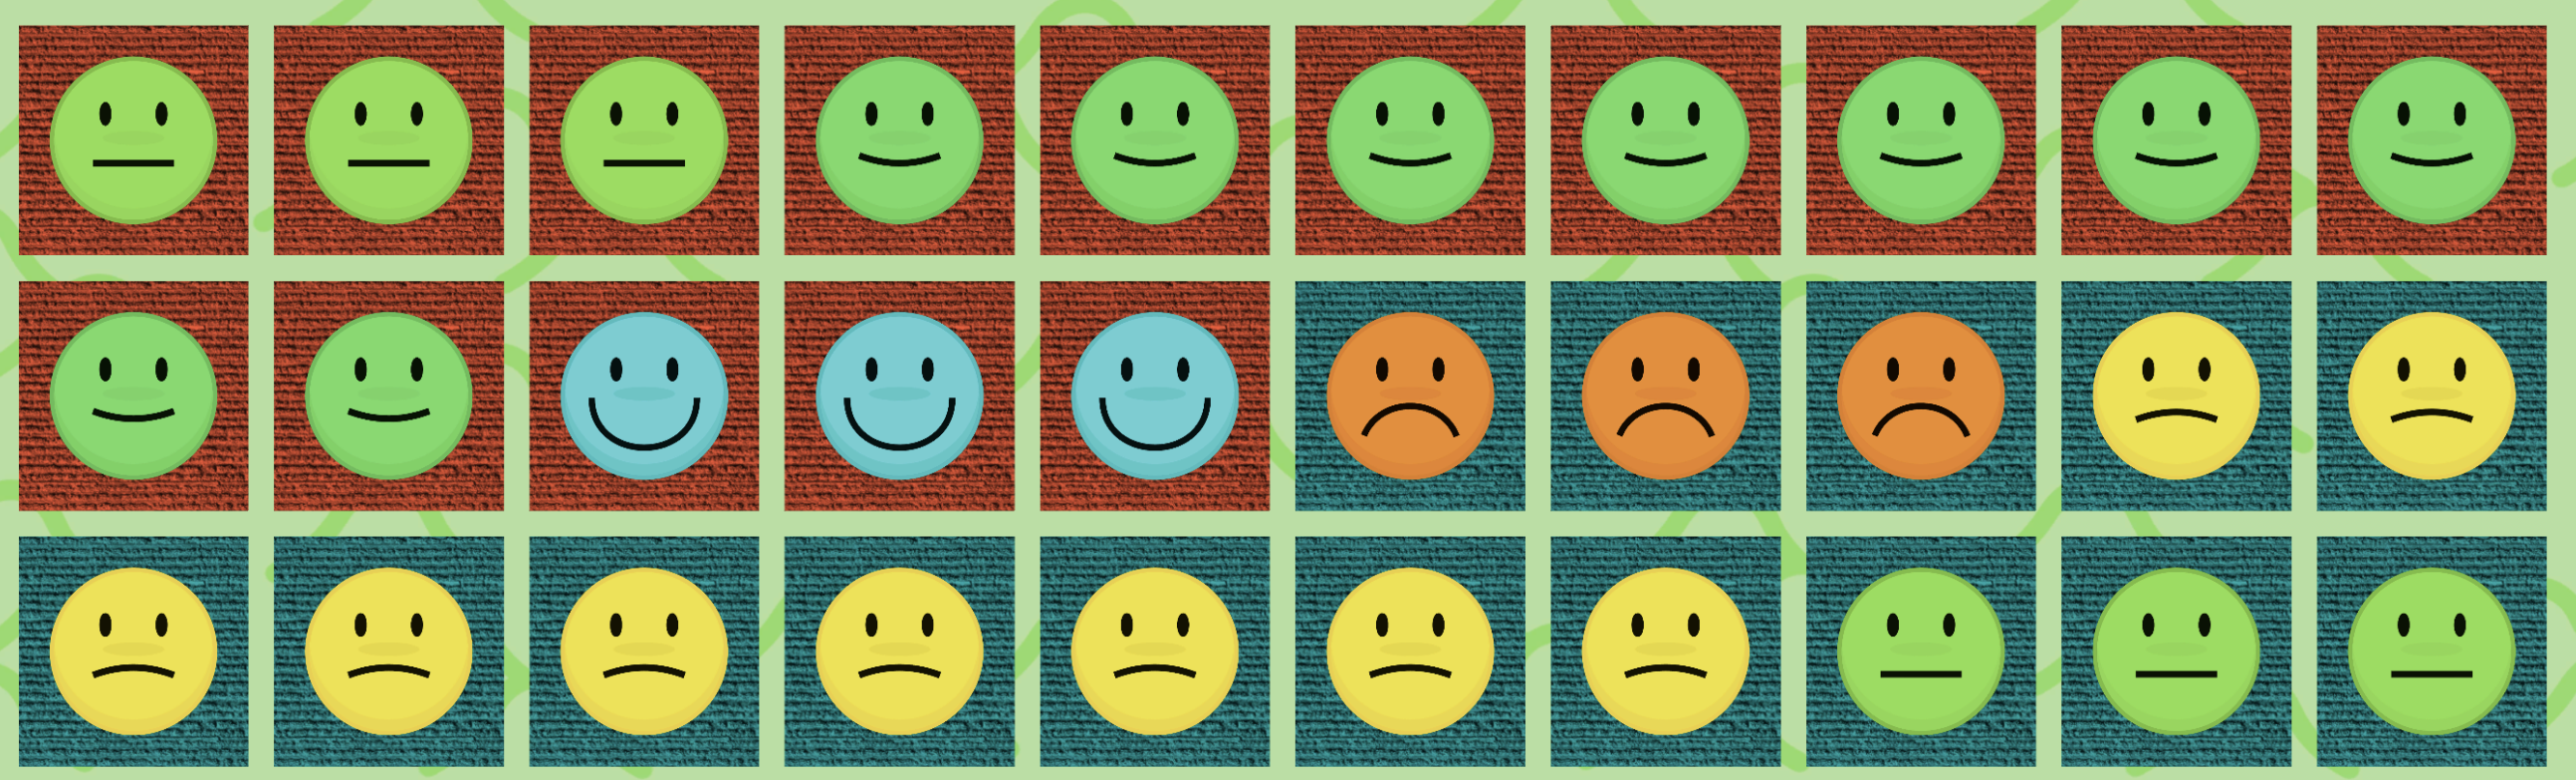
\includegraphics{game_halfway.png}

Where's the context uncertainty?

Where's the decision making?
\end{frame}

\begin{frame}{Adding Context Uncertainty}
\protect\hypertarget{adding-context-uncertainty}{}
Some characters have unknown type

They appear as gray

Could be either type

\begin{figure}

{\centering 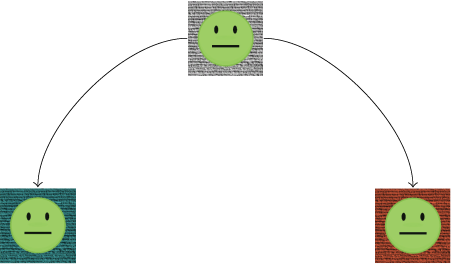
\includegraphics[width=5.72917in,height=3.125in]{gray_uncertainty.png}

}

\end{figure}
\end{frame}

\begin{frame}{Deciding Adoption Intensity}
\protect\hypertarget{deciding-adoption-intensity}{}
Land divided into 10 rows

Must decide adoption maximizing yield

Mapped to Likert Scale

\begin{figure}

{\centering 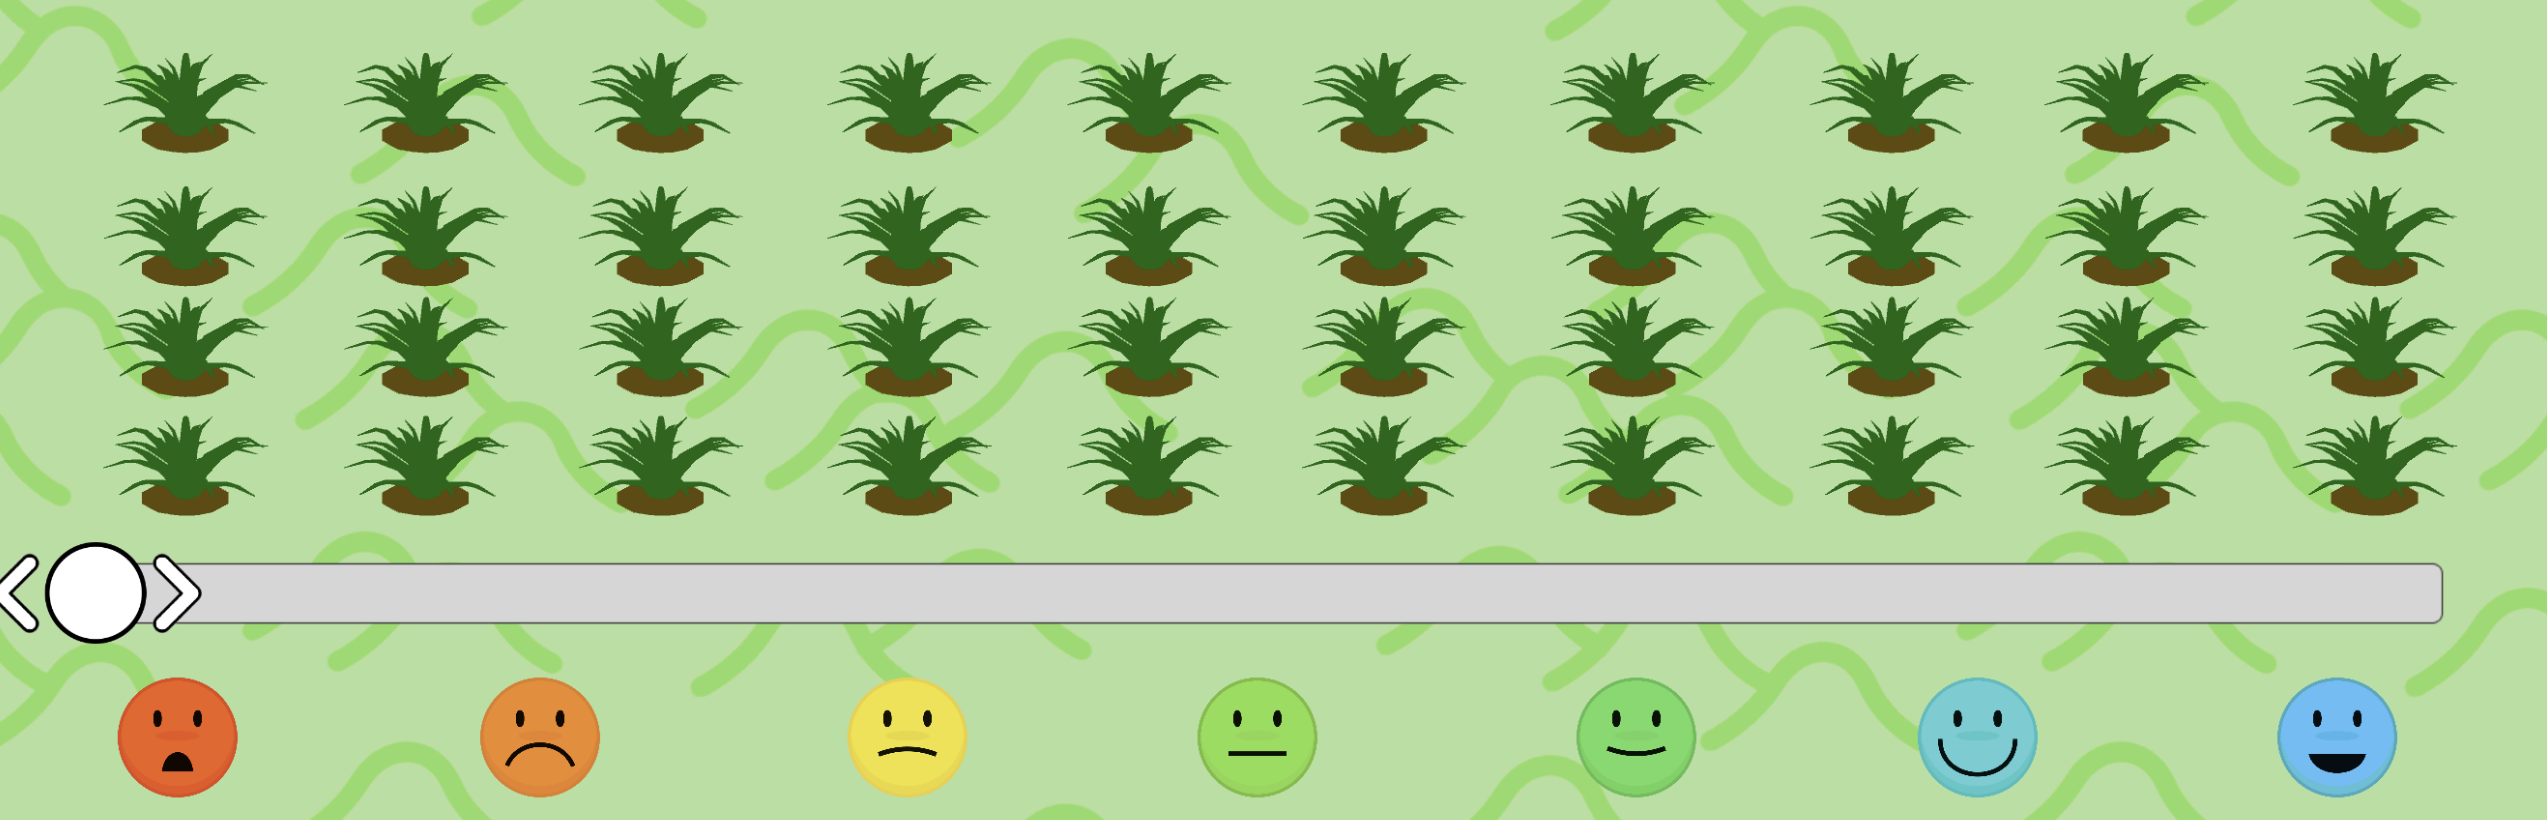
\includegraphics{adoption_choice.png}

}

\end{figure}
\end{frame}

\begin{frame}{Bringing it all together}
\protect\hypertarget{bringing-it-all-together}{}
Player sees information and decides adoption level

\begin{figure}

\begin{minipage}[t]{0.50\linewidth}

{\centering 

\raisebox{-\height}{

\includegraphics[width=5.20833in,height=\textheight]{game_5.png}

}

}

\end{minipage}%
%
\begin{minipage}[t]{0.50\linewidth}

{\centering 

\raisebox{-\height}{

\includegraphics[width=5.20833in,height=\textheight]{game_13.png}

}

}

\end{minipage}%

\end{figure}
\end{frame}

\begin{frame}{Process and Randomization}
\protect\hypertarget{process-and-randomization}{}
\begin{enumerate}[<+->]
[(1)]
\tightlist
\item
  Survey participant
\item
  Read game script
\item
  Practice module
\item
  Game modules

  \begin{itemize}[<+->]
  \tightlist
  \item
    Randomize round order via matched quartets
  \item
    Randomize technology order
  \item
    Randomize village name order
  \end{itemize}
\item
  Payout
\end{enumerate}
\end{frame}

\begin{frame}{Results}
\protect\hypertarget{results}{}
\end{frame}

\begin{frame}{How Context Uncertainty Aversion Is Tested}
\protect\hypertarget{how-context-uncertainty-aversion-is-tested}{}
\textbf{Identification:} Two game rounds. Only change \% gray

\begin{figure}

\begin{minipage}[t]{0.50\linewidth}

{\centering 

\raisebox{-\height}{

\includegraphics[width=5.20833in,height=\textheight]{game_5.png}

}

}

\end{minipage}%
%
\begin{minipage}[t]{0.50\linewidth}

{\centering 

\raisebox{-\height}{

\includegraphics[width=5.20833in,height=\textheight]{game_13.png}

}

}

\end{minipage}%

\end{figure}

\textbf{Specification:} \[
AdoptionLevel_{it} = \beta_1 \cdot \mathbb{1}_{t = \text{High } \% \text{ Gray}} + \eta_i + \epsilon_{it}
\]
\end{frame}

\begin{frame}{Farmers Prefer More Context}
\protect\hypertarget{farmers-prefer-more-context}{}
\begin{figure}

{\centering 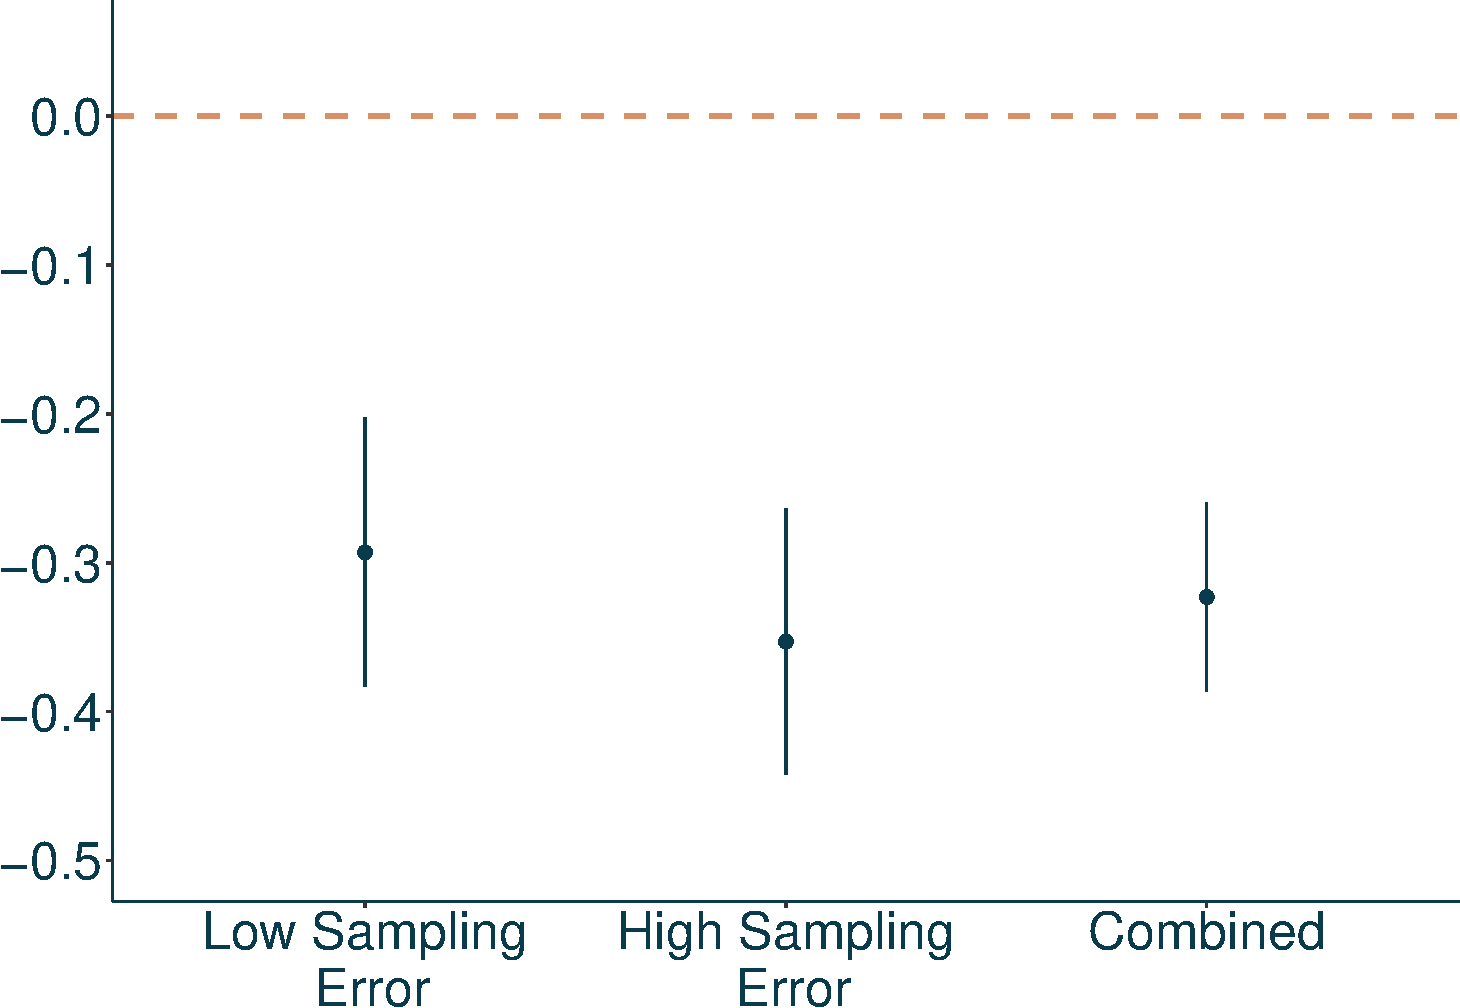
\includegraphics{presentation_lori_files/figure-beamer/unnamed-chunk-3-1.pdf}

}

\end{figure}

\begin{block}{Shifts in Adoption}
\protect\hypertarget{shifts-in-adoption}{}
\begin{figure}

{\centering 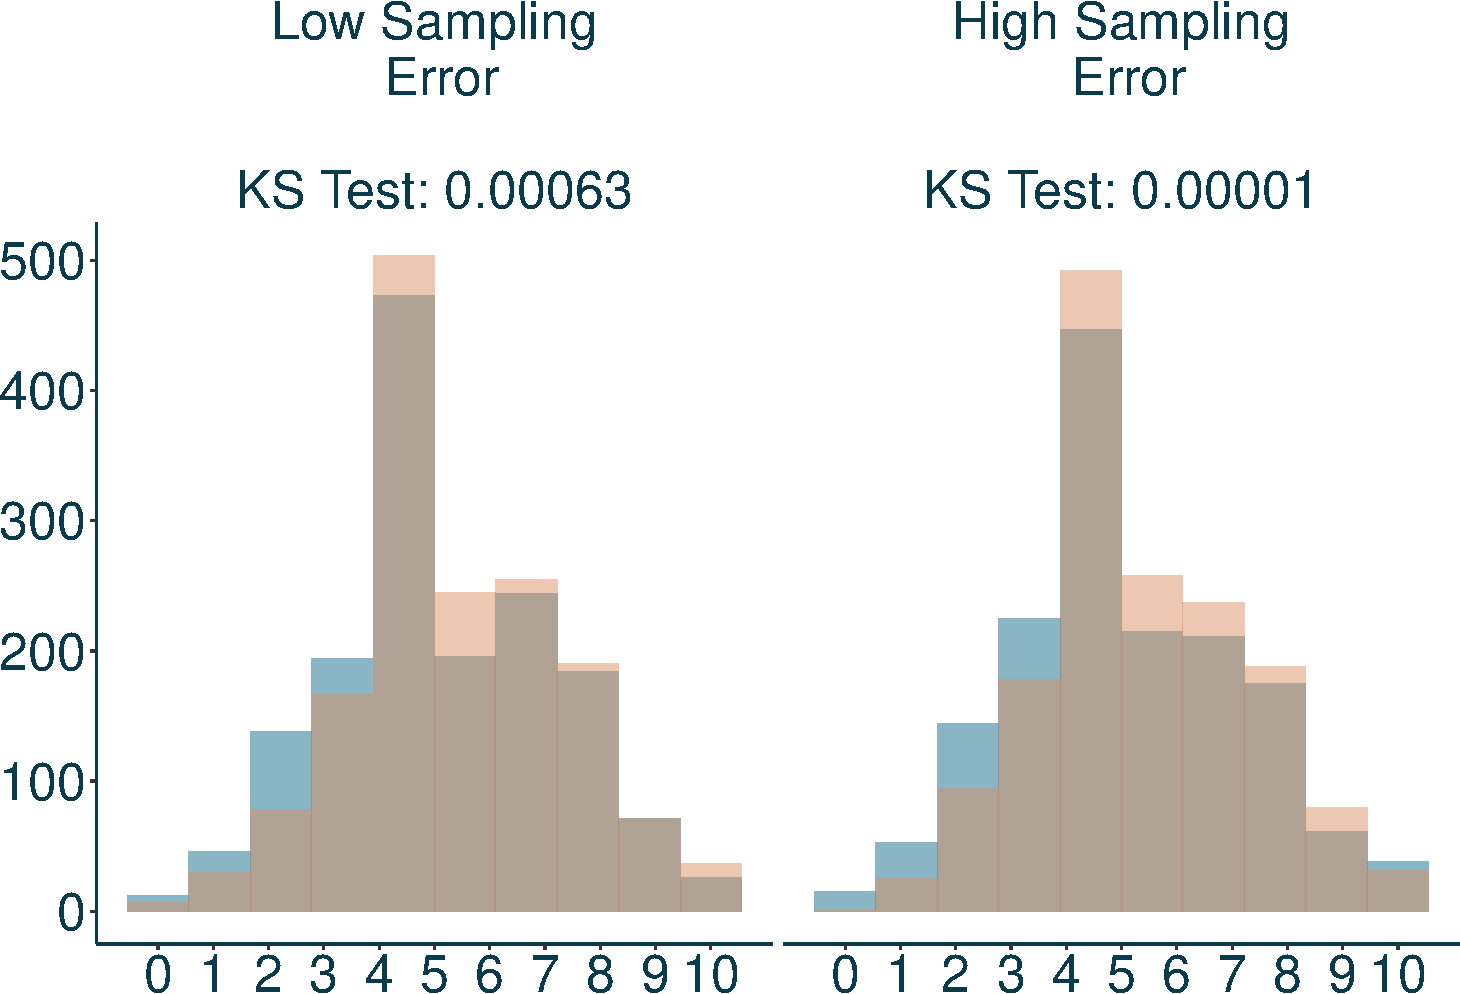
\includegraphics{presentation_lori_files/figure-beamer/unnamed-chunk-4-1.pdf}

}

\end{figure}
\end{block}
\end{frame}

\begin{frame}{How Complementarity Is Tested}
\protect\hypertarget{how-complementarity-is-tested}{}
\textbf{Identification:} Two modules. Low vs high sampling error.

\begin{figure}

\begin{minipage}[t]{0.50\linewidth}

{\centering 

\raisebox{-\height}{

\includegraphics[width=4.16667in,height=\textheight]{game_5.png}

}

}

\end{minipage}%
%
\begin{minipage}[t]{0.50\linewidth}

{\centering 

\raisebox{-\height}{

\includegraphics[width=4.16667in,height=\textheight]{game_14.png}

}

}

\end{minipage}%

\end{figure}

Change \% gray within each.

\begin{figure}

\begin{minipage}[t]{0.50\linewidth}

{\centering 

\raisebox{-\height}{

\includegraphics[width=4.16667in,height=\textheight]{game_13.png}

}

}

\end{minipage}%
%
\begin{minipage}[t]{0.50\linewidth}

{\centering 

\raisebox{-\height}{

\includegraphics[width=4.16667in,height=\textheight]{game_15.png}

}

}

\end{minipage}%

\end{figure}
\end{frame}

\begin{frame}{How Complementarity Is Tested}
\protect\hypertarget{how-complementarity-is-tested-1}{}
\textbf{Specification:} Use diff-in-diff (i.e.~Athey and Stern, 1998)

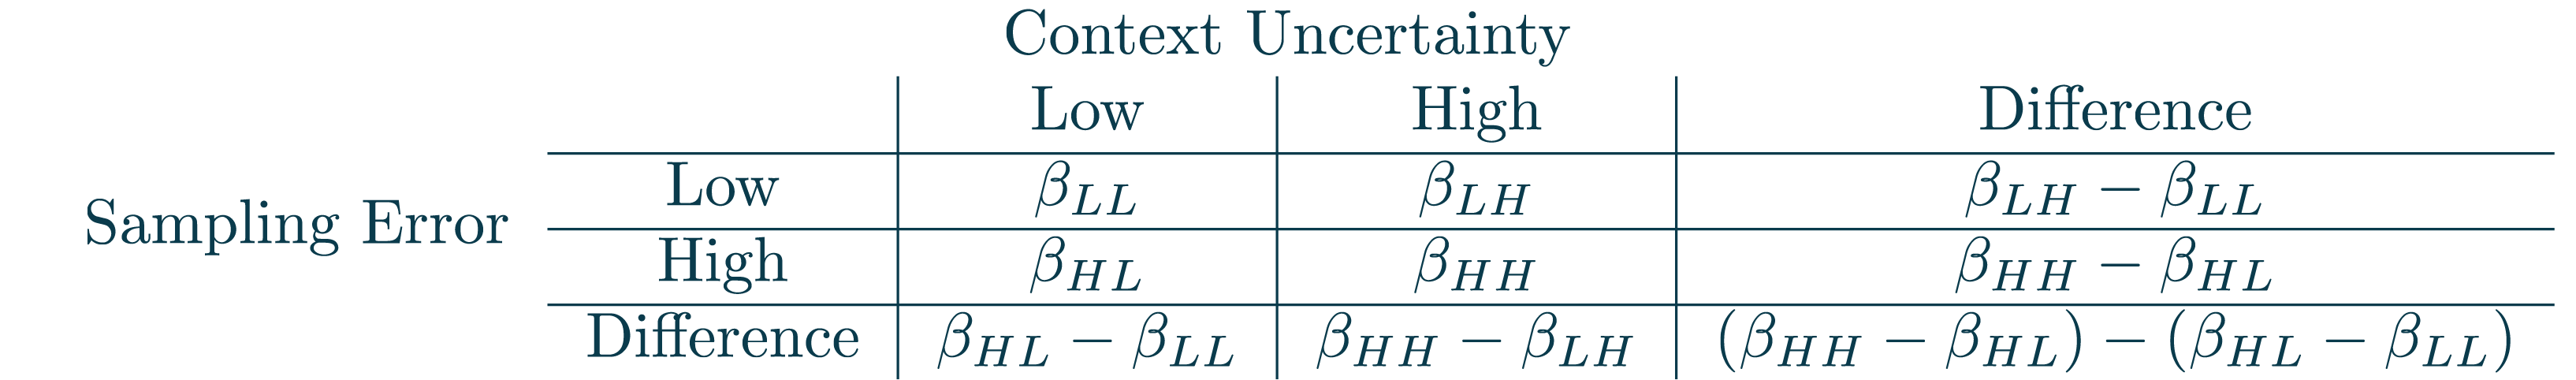
\includegraphics[width=15.625in,height=\textheight]{diffindifftab.png}

$$
AdoptionLevel_{it} =  \text{Whoops!} + \eta_i + \epsilon_{it}
$$

\end{frame}

\begin{frame}{Uncertainties May Be Complementary}
\protect\hypertarget{uncertainties-may-be-complementary}{}
\begin{figure}

{\centering \includegraphics{presentation_lori_files/figure-beamer/unnamed-chunk-5-1.pdf}

}

\end{figure}

\begin{block}{Dropped Enumerators Improve Significance}
\protect\hypertarget{dropped-enumerators-improve-significance}{}
\begin{figure}

{\centering \includegraphics{presentation_lori_files/figure-beamer/unnamed-chunk-6-1.pdf}

}

\end{figure}
\end{block}
\end{frame}

\begin{frame}{External Validity: Survey Evidence}
\protect\hypertarget{external-validity-survey-evidence}{}
\end{frame}

\begin{frame}{Farmers Consider Extension Agents Less Than Peers}
\protect\hypertarget{farmers-consider-extension-agents-less-than-peers}{}
59\% of farmers consider a peer more useful.

\textbf{Why?}

\begin{itemize}[<+->]
\tightlist
\item
  \(97\%\) cite less experience
\item
  \(> 40\%\) cite more heterogeneity (budget, land, resources)
\item
  Only \(5\%\) suspect ulterior motives (i.e.~corruption)
\end{itemize}

\begin{figure}

{\centering \includegraphics{presentation_lori_files/figure-beamer/unnamed-chunk-7-1.pdf}

}

\end{figure}

\begin{frame}{Farmers Strongly Prefer Similar Test Plots}
\protect\hypertarget{farmers-strongly-prefer-similar-test-plots}{}
\begin{figure}

{\centering \includegraphics{presentation_lori_files/figure-beamer/unnamed-chunk-8-1.pdf}

}

\end{figure}
\end{frame}



\end{document}
